\documentclass[journal]{IEEEtran}

\usepackage{ifpdf}
\usepackage{multirow}
\usepackage{multicol}
\usepackage{booktabs}
\usepackage{cite}
\usepackage[normalem]{ulem}
\usepackage{xcolor}
\ifCLASSINFOpdf
  \usepackage[pdftex]{graphicx}
\else
  \usepackage[dvips]{graphicx}
\fi
\graphicspath{{figures/}{analysis/plots/}}
\usepackage{amsmath}
\usepackage{amssymb}
\usepackage{algorithm}
\usepackage{algpseudocode}
\usepackage{array}
\usepackage{float}
\ifCLASSOPTIONcompsoc
  \usepackage[caption=false,font=normalsize,labelfont=sf,textfont=sf]{subfig}
\else
  \usepackage[caption=false,font=footnotesize]{subfig}
\fi
\usepackage{fixltx2e}
\usepackage{stfloats}
\usepackage{url}

\begin{document}

\title{The Cost of Tactile Sensing at Training Scale:\ Four Representations, a Contact-Budget Trap, and a Sparse GPU Encoder}

\author{Afthab Shiraz, University College London}

\maketitle

\begin{abstract}
This report measures what a hardware-faithful tactile observation costs in a GPU-parallel MuJoCo Warp simulation of the LeapXELA hand, across the four representations available to the project, and then removes the cost of the one worth keeping. At the training timestep of 0.01~s and 4096 parallel environments the four differ by more than two orders of magnitude. Native MuJoCo \texttt{\textless touch\textgreater} sensing (421 sensors) is a 1.7\% throughput tax and is already on GPU. A faithful dense PyTorch port of the three-channel, 368-taxel Gaussian-splat encoder used by the reference XELA software multiplies step cost by 4.57 and occupies 76.9\% of step time. A 300-patch binary touch grid costs 4.35 and cannot be run at the reference contact budget at all. A deformable flex skin runs on MuJoCo Warp, where the JAX backend refuses it outright, but at its own required timestep of 0.002~s is roughly 540 times slower than the rigid hand at matched simulated time, and saturates early. The splat is therefore the representation worth optimising, and profiling shows it is bandwidth-bound rather than compute- or launch-bound: arithmetic intensity is 0.192~FLOP/byte against an empirically measured ridge point of 70.7~FLOP/byte. A two-pass Triton gather kernel avoids dense environment--contact--taxel intermediates and reduces modeled traffic from 19.99~GB to 136~MB; it is 188 times faster than eager PyTorch and 78 times faster than \texttt{torch.compile} in isolation, and end to end reduces the cost of touch from 4.57 to 1.09 times the physics-only step, 96\% of a 4.34-fold Amdahl ceiling. Replacing the frozen benchmark pose with seven scripted grasp patterns, decorrelated across worlds, leaves that result intact at 1.01. The touch-grid measurement partly refutes this study's own registered hypothesis: the extra contacts are nearly free, while the contact budget that must be allocated to hold them is not. Step time is affine in allocated \texttt{nconmax} at fixed occupancy, which makes \texttt{nconmax} a first-class throughput parameter worth 3.4-fold at 1024 environments rather than a safety margin. Wired into the reference training environment itself, with its managers, resets and randomisation, the encoder costs 1.19 times a tactile-free step at 2048 environments, corroborating the isolated benchmark; reaching that figure required fixing an unrelated accessor in the RL framework worth a further 3.31-fold. Throughputs are reported as physics steps per second; the reference environment's decimation of five converts them to control steps. The study covers the simulator step rather than a complete policy-training loop, and those boundaries are kept explicit.
\end{abstract}

\begin{IEEEkeywords}
Tactile sensing, GPU simulation, MuJoCo Warp, Triton, reinforcement learning, performance engineering.
\end{IEEEkeywords}

\IEEEpeerreviewmaketitle

\section{Introduction}

\IEEEPARstart{G}{PU-parallel} simulation amortises control and physics work across thousands of independent robot environments. This makes quantities that were negligible in a single environment candidates for the dominant cost at training scale. Tactile hands are a particularly relevant case: the physical sensor may expose hundreds of spatially arranged measurements, while a simulator must derive those measurements from an irregular and changing contact set every step.

The target system is the rigid LeapXELA hand used by the supervisor's mjlab cube-reorientation stack. Its existing observations contain no tactile term. Four ways of supplying one were available, and they are not variations on a theme: they place their cost in different parts of the simulator, and they differ by more than two orders of magnitude at training scale. Native MuJoCo \texttt{\textless touch\textgreater} sensors are a scalar-per-zone readout that MuJoCo Warp already executes on GPU inside the step. The associated CPU software provides \texttt{VirtualTaxelSensor}, a hardware-faithful Gaussian-splat encoder whose 368 three-axis outputs preserve the ordering of the physical XELA taxels; it consumes the contact set after physics and had no GPU implementation. A binary touch grid tiles the hand with small collision geoms and therefore charges its cost to contact generation rather than to a readout. A deformable flex skin resolves contact against a simulated membrane and charges its cost to the solver.

Framing the work as a comparison rather than as a single optimisation is what makes the optimisation meaningful. A kernel that removes a 4.57-fold overhead is a speedup in a vacuum unless the alternatives are priced; once they are, it is the difference between the faithful representation being unaffordable and being roughly as cheap as the built-in one. Prior mjlab work with an 18-taxel Robotiq gripper reads built-in force sensors and does not supply this representation, kernel, or scaling study.

This work makes five contributions. First, it reconciles the separate tactile/CPU and RL/GPU hand-model lineages and injects the taxel sites into the pinned rigid model. Second, it builds a memory-capped benchmark and a faithful batched PyTorch baseline. Third, it establishes by profiling that the baseline is bandwidth-bound because it materialises dense intermediates that mostly carry no signal. Fourth, it implements and validates a sparse two-pass gather kernel; the principal systems result is bottleneck migration, in that the naive encoder overtakes physics at $N=256$ while the optimised encoder reduces its share at $N=4096$ from 76.9\% to 6.5\%. Fifth, it measures the other three representations under the same scene, timestep and memory isolation, which yields a cost-of-sensing comparison and one finding that generalises beyond tactile work: the throughput of a MuJoCo Warp step is affine in the \emph{allocated} contact budget and blind to how much of it is occupied.

\begin{figure}[t]
  \centering
  
\includegraphics[width=\columnwidth]{A_bottleneck_migration.png}
  \caption{Bottleneck migration at the supervisor's 0.01~s simulation timestep. The dense encoder overtakes physics at $N=256$ and dominates at larger batches.}
  \label{fig:migration}
\end{figure}

\section{Background}

\subsection{MuJoCo Warp and parallel environments}

MuJoCo Warp expresses MuJoCo dynamics as GPU kernels over many worlds. In this study the same closed-hand cube-reorientation scene is replicated across $N$ environments. Physics throughput initially scales nearly linearly because additional environments fill otherwise idle parallel capacity; after saturation, step latency grows but aggregate steps per second can continue to increase. Tactile encoding is performed after the contact state is available and therefore adds to the simulator step.

The tested machine is an aarch64 NVIDIA DGX Spark with a GB10 GPU and 48 streaming multiprocessors. CPU and GPU share unified LPDDR5X memory. This matters operationally: an excessive allocation can exhaust host memory and wedge the machine rather than produce an isolated device out-of-memory exception. It also means that the empirically measured bandwidth ceiling is a shared resource.

Warp also requires two static per-world budgets to be declared before allocation: \texttt{nconmax}, the number of contact slots, and \texttt{njmax}, the number of constraint rows. The reference configuration sets these to 48 and 120. Section~\ref{sec:grid} shows that the first of these is not a passive reservation.

\subsection{Throughput units}
\label{sec:units}

All throughputs in this report are \emph{physics} steps per second, aggregated over worlds: one \texttt{mjw.step} per environment per step. The reference environment configuration uses \texttt{ctrl\_dt}=0.05~s with \texttt{sim\_dt}=0.01~s, hence \texttt{decimation}=5, so one of its environment steps is five of the steps measured here. Any comparison with a training-loop rate must divide by five. At $N=4096$ the physics-only figure of 128,061 physics steps/s corresponds to 25,612 control steps/s, and the Triton-encoded figure of 116,961 corresponds to 23,392. The ratios reported throughout --- cost of touch, encoder share, speedup --- are unaffected by the conversion, since numerator and denominator carry the same factor.

\subsection{Four tactile representations}

\emph{Native \texttt{\textless touch\textgreater}.} MuJoCo's built-in touch sensor sums the normal force of contacts falling inside a sensor zone and reports one scalar per zone. Warp evaluates it inside \texttt{mjw.step} over a launch dimensioned by the allocated contact budget and the sensor count. The injected model used here carries 421 such sensors.

\emph{Gaussian splat.} The reference CPU encoder described below. It is a post-physics readout: it consumes contact positions and forces and produces $368\times3$ floats per environment.

\emph{Binary touch grid.} The hand is tiled with 300 small patch geoms, each of which reports whether it is currently in contact. It produces no readout arithmetic worth measuring; its cost lives entirely inside contact generation and constraint solution, which is why it is the representation that interacts with the budgets above.

\emph{Flex skin.} A deformable membrane over the hand, in the tactile lineage's 387-body, 1120-joint, 18-flex model with 386 equality constraints. It is the most physically faithful and the only one whose cost falls on the solver.

\subsection{The Gaussian-splat representation}

For each valid object--hand contact, the reference encoder obtains the linear contact force, applies the contact-frame rotation and sign convention, and considers only taxels belonging to the contacted body. For taxel $t$ and contact $c$, the contact offset is transformed into the taxel-local frame. Writing the local offset as $(x_{ct},y_{ct},z_{ct})$, the unnormalised weight is
\begin{equation}
  w_{ct}=\exp\left(-\frac{x_{ct}^{2}+y_{ct}^{2}}{2\sigma^{2}}\right).
\end{equation}
The weight is set to zero outside the in-plane cutoff and when $|z_{ct}|$ exceeds the same cutoff. This latter patch-locality gate prevents a contact from splatting onto a different patch that happens to share a rigid body. The remaining weights are normalised independently for each contact over that body's taxels. The locally rotated force is then accumulated into three output channels per taxel, with the normal sign changed so compression is positive.

The calculation is irregular in two ways. The number and body assignment of contacts change with state, and different bodies own different subsets of taxels. A direct batch formulation regularises the shapes by padding every environment to 48 contact slots and evaluating all 368 taxels. It is simple and faithful, but creates a dense $B\times C\times T$ product whose work grows with $B$ even though only live contacts and the contacted body's taxels can contribute.

\section{Method}

\subsection{Model reconciliation and taxel injection}
\label{sec:method-model}

The RL/GPU model and tactile/CPU model are distinct lineages and the 12 layout bodies share zero names with the RL model. A name-order mapping would also be wrong: the tactile lineage's body named \texttt{finger} is the ring finger, not the index finger, so the apparently natural ordering silently swaps the ring and index chains. The mapping was instead derived from the kinematic tree, disambiguated by hardware patch names, and checked using body-local mesh bounding boxes. The palm and all proximal and middle links agree exactly under that check. The four fingertips differ geometrically; this limitation is discussed in Section~\ref{sec:threats}.

The two lineages are more closely related than their disjoint body names suggest, which sharpens what that fingertip difference means. Both ship a mesh asset directory, and 17 \texttt{.stl} filenames occur in both: all 17 carry identical triangle counts and \textbf{10 are byte-for-byte identical}. Independent exports do not produce identical files, so these are two exports of one CAD project rather than two separate modelling efforts. The files that do differ are re-exports --- same triangle count, same bounding box to 0.01~mm, vertices differing by at most 1.5~mm. Against that background the fingertip stands out as the single component that shares no filename at all: the RL lineage's \texttt{fingertop\_unfied.stl} measures 72.31~mm along its long axis where the tactile lineage's \texttt{fingertip\_fix.stl} measures 61.98~mm. The 10.33~mm discrepancy is therefore one revised part captured at two revisions, not an unresolvable disagreement between two models, and it has a definite answer that the model's author can supply.

The 368 sites are injected into the pinned 17-body rigid model using MuJoCo's specification API. Per-body ray tests show that every injected site remains within the reference encoder's patch-locality gate. Remapping the layout is essential as well as injecting sites: without it, reference body lookups return an invalid identifier, all taxels collapse into a bogus group, and the encoder produces plausible-looking all-zero output without raising an error.

\subsection{Oracle and correctness gates}

The CPU \texttt{VirtualTaxelSensor} supplied with the tactile model is treated as the semantic oracle. A banked fixture contains the inputs and 368-by-3 outputs for a scripted grasp, including no-contact frames, so implementations can be compared without introducing CPU-versus-Warp contact-generation differences. The reference accumulates in double precision and casts at its output, whereas the GPU paths use single precision; agreement is therefore assessed by measured absolute error rather than bit equality with the oracle.

The batched PyTorch implementation preserves the reference operations: contact-force rotation, body masking, Gaussian and locality gates, per-contact normalisation, local-force rotation, accumulation, and the final normal sign. It deliberately creates the dense intermediates and serves as a readable baseline. The Triton implementation is gated both against the oracle and against this baseline, including empty contacts, zero normalisers, invalid padded slots, and contacts on bodies with no taxels.

\subsection{Memory-capped benchmark harness}

Every environment count runs in a separate subprocess under a systemd memory scope. Subprocess isolation both releases allocator state between points and ensures that the memory controller kills only the child if a run exceeds its cap. The harness warms the simulator, synchronises Warp on both sides of timing, and records fused throughput separately from a stage-synchronised physics/encoder decomposition. Physics-only, native-touch, touch-grid, eager-splat, and Triton-splat sweeps use the same scene, timestep and solver settings. \texttt{nconmax} and \texttt{njmax} are command-line parameters rather than constants, which is what makes it possible to hold the physics fixed and vary only the declared budget. This report uses only the \texttt{\_dt01.csv} sweeps, for which the model timestep is explicitly set to 0.01~s to match the supervisor's configuration; earlier unsuffixed sweeps inherited 0.001~s and are superseded for end-to-end reporting.

\subsection{Comparing representations in one scene}

Three of the four representations are measured in the same pinned rigid scene, so their throughputs are directly comparable. The native touch sensors are \emph{injected} into that scene rather than read from the standalone reference touch model, which reports exactly zero: its sensor pads were reduced to visual meshes, leaving the nearest contact 9.42~mm from a 1.00~mm sensor zone. The 300 patch geoms are likewise injected, taking the scene from 71 to 371 geoms.

Native touch has no separable stage to time, because Warp evaluates it inside \texttt{mjw.step}. Its cost is therefore obtained as a difference of fused loops with the sensors present and absent, and is reported against an explicitly measured timing-noise floor.

Flex is the exception and is measured by a separate probe, \texttt{benchmarks/flex\_probe.py}. The flex hand is a different body tree in the tactile lineage; unlike taxel sites and patch geoms there is no injection that converts one model into the other. Its per-step latency is therefore a same-engine, same-timestep, same-GPU order-of-magnitude comparison, and its throughput is not a like-for-like fourth bar. Section~\ref{sec:threats} restates that limit.

\subsection{Frozen pose and grasp motion}
\label{sec:motion}

The sweeps were first taken at a single frozen operating point: all 16 actuators driven to 60\% of range in every world, the cube settled, and the pose then held for the whole timed region. That produces a stable and reproducible contact regime averaging 7.5 contacts per environment, but it is a weak test of a data-dependent kernel, because every world sits at the same moderate occupancy for the entire measurement --- none is idle and none is loaded.

Every sweep was therefore repeated under motion. Seven grasp patterns were ported from the supervisor's own tactile data-collection code, with the pattern shapes, timings and fractions copied verbatim rather than re-tuned. World $w$ runs pattern $w \bmod 7$ at a phase offset, so at any instant the population spans the full range of the motion. At $N=4096$ the measured per-world contact count ranges from 0 to 25, with a population mean of 7.3 against the frozen pose's 7.5. Contact statistics are sampled by replaying the same motion outside the timed region, since under motion the count is no longer a constant that a single post-run reading can characterise.

\subsection{Profiling method}

The eager encoder was measured with PyTorch's per-operation CUDA profiler and an Nsight Systems timeline. A code-derived cost model assigns bytes and floating-point operations to each operation. Hardware-counter profiling was attempted but unavailable, as detailed in Section~\ref{sec:threats}. Consequently, achieved bandwidth is modeled bytes divided by measured time. The comparison ceilings are empirical measurements on the same otherwise-idle host: 260.8~GB/s for a saturating read and 18.44~TFLOP/s for FP32 SGEMM with TF32 disabled.

The profiling diagnosis is tested experimentally by compiling the unmodified encoder. \texttt{torch.compile} changes neither algorithm nor sparsity, but fuses elementwise work and removes intermediate round trips. Its 2.41-fold isolated speedup at $N=4096$, with numerically identical output at the reported tolerance, is both a useful baseline and a controlled test of the traffic diagnosis.

\subsection{Two-pass gather kernel}

The Triton design assigns pass 1 to contact normalisation and pass 2 to taxel output. Pass 1 uses one program per environment--contact pair, visits only taxels on the contacted body, and stores one weight sum. Pass 2 uses one program per environment--taxel tile, traverses contact slots in fixed order, recomputes the Gaussian weights, and accumulates the three force channels in registers. It emits only the final output; no $B\times C\times T$ intermediate is materialised.

The two-pass form is forced by the mathematics rather than selected merely to reduce launches. Normalisation divides each weight by a reduction over the taxel axis, but that taxel axis is the parallel axis of the gather pass. Its denominator must therefore be available before pass 2 consumes it. Storing every weight would reintroduce substantial traffic, so the kernel stores one scalar normaliser per contact and recomputes weights. This is appropriate on a workload whose measured arithmetic intensity lies far below the machine ridge point. Both passes use fixed traversal orders and no atomics.

\section{Results}

\subsection{The cost of four representations at training scale}
\label{sec:fourways}

Table~\ref{tab:fourways} is the study's summary measurement, and Fig.~\ref{fig:fourways} shows the comparable subset of it. At $N=4096$ and the training timestep, the four ways of obtaining a tactile observation span more than two orders of magnitude, and the spread is structural rather than a matter of tuning: each representation charges its cost to a different part of the simulator.

\begin{table}[t]
\caption{Cost of tactile sensing at $N=4096$ and $\mathit{sim\_dt}=0.01$~s, frozen benchmark pose. Rates are physics steps/s aggregated over worlds; divide by the reference \texttt{decimation}=5 for control steps. Cost of touch is the physics-only rate divided by the row's rate.}
\label{tab:fourways}
\centering
\small
\begin{tabular}{lrrrr}
\toprule
Representation & Outputs & \texttt{nconmax} & Steps/s & Cost \\
\midrule
None (physics only) & ---   & 48  & 128,061 & 1.00$\times$ \\
Native \texttt{\textless touch\textgreater}  & 421   & 48  & 125,877 & 1.02$\times$ \\
Splat, Triton       & 1104  & 48  & 116,961 & 1.09$\times$ \\
Splat, dense PyTorch& 1104  & 48  & 28,006  & 4.57$\times$ \\
Binary touch grid   & 300   & 256 & 29,440  & 4.35$\times$ \\
Flex skin$^{\dagger}$ & ---  & 48  & ---     & $\approx$540$\times$ \\
\bottomrule
\end{tabular}

\vspace{2pt}
\footnotesize $^{\dagger}$ Different body tree; not directly comparable, so no rate is given. The ratio is at $N=256$ and at matched simulated time: flex's per-step latency is 107.6 times the rigid hand's, and its 0.002~s timestep advances one fifth as far as the 0.01~s used elsewhere. Flex is the only representation that has already stopped scaling by that point.
\end{table}

\begin{figure}[t]
  \centering
  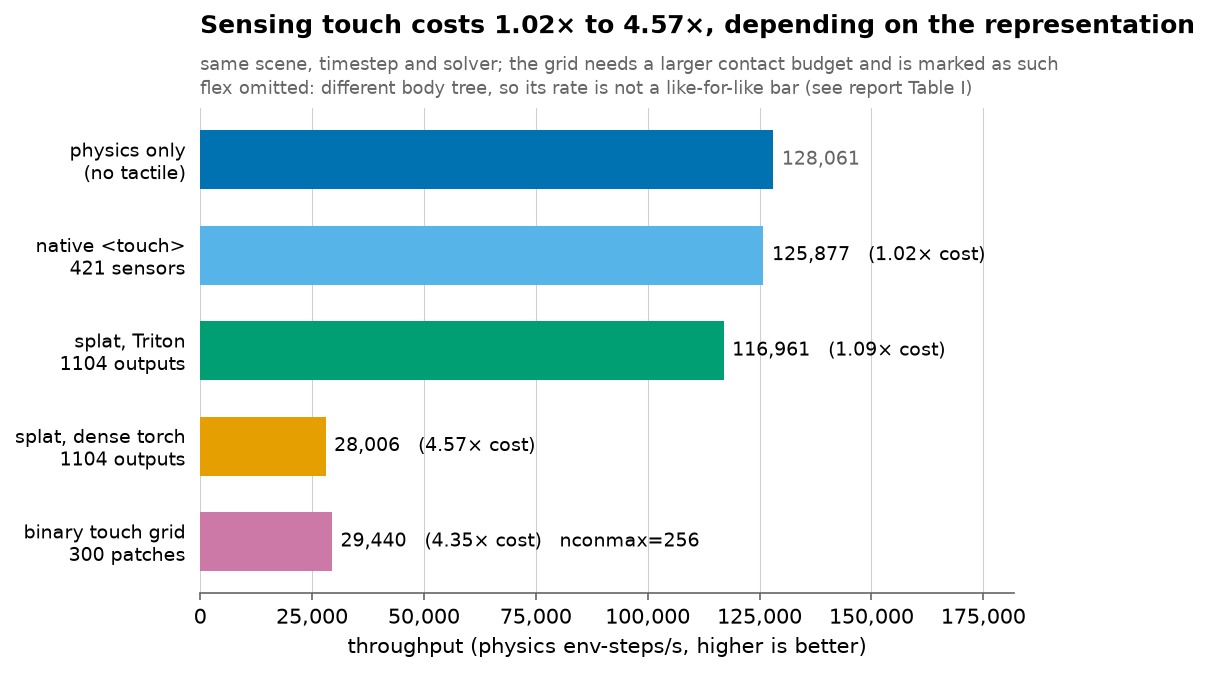
\includegraphics[width=\columnwidth]{I_four_representations.png}
  \caption{The comparable representations at $N=4096$, measured in one scene at one timestep. Flex is omitted rather than plotted: it is a different body tree, so its rate is not a like-for-like bar, and it appears only in Table~\ref{tab:fourways} where the caveat travels with the number. The touch grid is annotated with the larger contact budget it requires, which is itself the subject of Section~\ref{sec:grid}.}
  \label{fig:fourways}
\end{figure}

Three points are worth stating before the mechanisms are unpacked. First, native touch is essentially free. Its end-to-end cost at $N=4096$ is 1.7\% of throughput. Isolating it by differencing fused loops, the touch dispatch itself is below the measured timing-noise floor at most environment counts and resolves only at the largest two: 0.037~ms against a $\pm$0.015~ms floor at $N=1024$ and 0.308~ms against $\pm$0.047~ms at $N=4096$, that is 0.3\% and 1.0\% of the step, with the readout adding a further 0.007 and 0.045~ms. The end-to-end figure is larger than that sum, which is the expected relationship when the effect being measured is close to run-to-run variation; at $N=256$ and $N=1024$ the touch-enabled sweep is nominally \emph{faster} than the physics-only sweep.

The conclusion survives the grasp motion of Section~\ref{sec:motion}. Under the seven decorrelated patterns at $N=4096$, native touch measures 117,601 physics steps/s against a moving physics-only baseline of 126,637, a cost of 1.08. Its differenced dispatch cost rises to 1.155~ms against a $\pm$0.126~ms noise floor, where the frozen pose gave 0.308~ms, although the mean contact count is essentially unchanged at 7.3 per environment; since both figures are differences of separately timed fused loops, the increase is more safely read as the spread of that estimator than as a motion effect. The mid-range rungs remain noise-dominated in the same way as at the frozen pose --- at $N=1024$ the touch sweep again measures nominally faster than physics-only, 87,680 against 72,804 --- so 1.08 bounds the cost rather than resolving it. If a scalar-per-zone readout is sufficient for a task, it is already available on GPU at a price that is hard to measure, moving or still.

Second, the two expensive representations are expensive for unrelated reasons. The dense splat is expensive after physics, in memory traffic (Section~\ref{sec:profiling}). The touch grid is expensive inside physics, and not in the way its registered hypothesis predicted (Section~\ref{sec:grid}). Their similar 4.6-fold and 4.3-fold costs are a coincidence of magnitude.

Third, only one of the two admits a kernel fix. The splat's cost is in code this project controls and is removed by rewriting it; the touch grid's cost is in mujoco\_warp's launch dimensions and cannot be reached from a readout kernel at all.

\subsection{Scaling and first bottleneck migration}

Table~\ref{tab:scaling} reports selected current sweep points. Physics-only latency is approximately flat through $N=128$, while aggregate throughput rises with $N$; saturation begins between 128 and 256 environments. The dense encoder's share then rises with scale. It crosses 50\% at $N=256$ and reaches 76.9\% at $N=4096$, confirming the registered crossover range. Figure~\ref{fig:throughput} shows the corresponding throughput scaling, and Fig.~\ref{fig:share} isolates the change in encoder share.

\begin{table}[t]
\caption{Current scaling results at $\mathit{sim\_dt}=0.01$~s. Rates are physics steps/s (Section~\ref{sec:units}); encoder shares come from stage-synchronised measurements.}
\label{tab:scaling}
\centering
\small
\begin{tabular}{rrrrr}
\toprule
$N$ & Physics & Eager & Triton & Eager share \\
\midrule
64   & 15,999  & 11,264 & 13,960  & 27.7\% \\
256  & 38,310  & 18,486 & 34,715  & 53.3\% \\
1024 & 78,349  & 25,148 & 77,361  & 70.2\% \\
4096 & 128,061 & 28,006 & 116,961 & 76.9\% \\
\bottomrule
\end{tabular}
\end{table}

\begin{figure}[t]
  \centering
  
\includegraphics[width=\columnwidth]{B_throughput_scaling.png}
  \caption{Aggregate throughput continues to improve after physics saturation, but the dense splat path separates sharply from the physics-only and Triton paths at large $N$.}
  \label{fig:throughput}
\end{figure}

\begin{figure}[t]
  \centering
  
\includegraphics[width=\columnwidth]{C_encoder_share.png}
  \caption{The eager encoder becomes the majority of stage-synchronised step time at $N=256$; the Triton encoder remains a small fraction at the largest batch.}
  \label{fig:share}
\end{figure}

\subsection{Profiling verdict}
\label{sec:profiling}

At $N=4096$, the eager encoder moves 19.99~GB according to the operation-level traffic model and performs 3.843~GFLOP, for an arithmetic intensity of 0.192~FLOP/byte. The empirical ridge point is 70.7~FLOP/byte, placing the workload 368-fold to the bandwidth side of the ridge. It achieves 35.3~GFLOP/s, only 0.19\% of the measured compute ceiling. Conversely, modeled traffic divided by runtime is 183.9~GB/s, or 71\% of the measured read ceiling. The elementwise subset reaches 87\% of that ceiling.

Launch overhead is not material: 58 launches at 3.34~$\mu$s account for 0.194~ms, or 0.18\% of the call. The dense product evaluates 72.4 million environment--contact--taxel triples, while measured contact sparsity and body masking leave about 492 thousand carrying signal. Thus the problem is not too little fusion alone; the algorithm visits and materialises predominantly irrelevant pairs. Table~\ref{tab:profile} summarises the evidence.

\begin{table}[t]
\caption{Profiling evidence at $N=4096$. Achieved bandwidth is modeled traffic divided by measured time, not a hardware-counter reading.}
\label{tab:profile}
\centering
\small
\begin{tabular}{lr}
\toprule
Metric & Value \\
\midrule
Eager traffic & 19.99~GB \\
Eager arithmetic & 3.843~GFLOP \\
Arithmetic intensity & 0.192~FLOP/byte \\
Measured ridge point & 70.7~FLOP/byte \\
Modeled achieved bandwidth & 183.9~GB/s \\
Measured read ceiling & 260.8~GB/s \\
Measured FP32 ceiling & 18.44~TFLOP/s \\
Launch-overhead share & 0.18\% \\
\bottomrule
\end{tabular}
\end{table}

\begin{figure}[t]
  \centering
  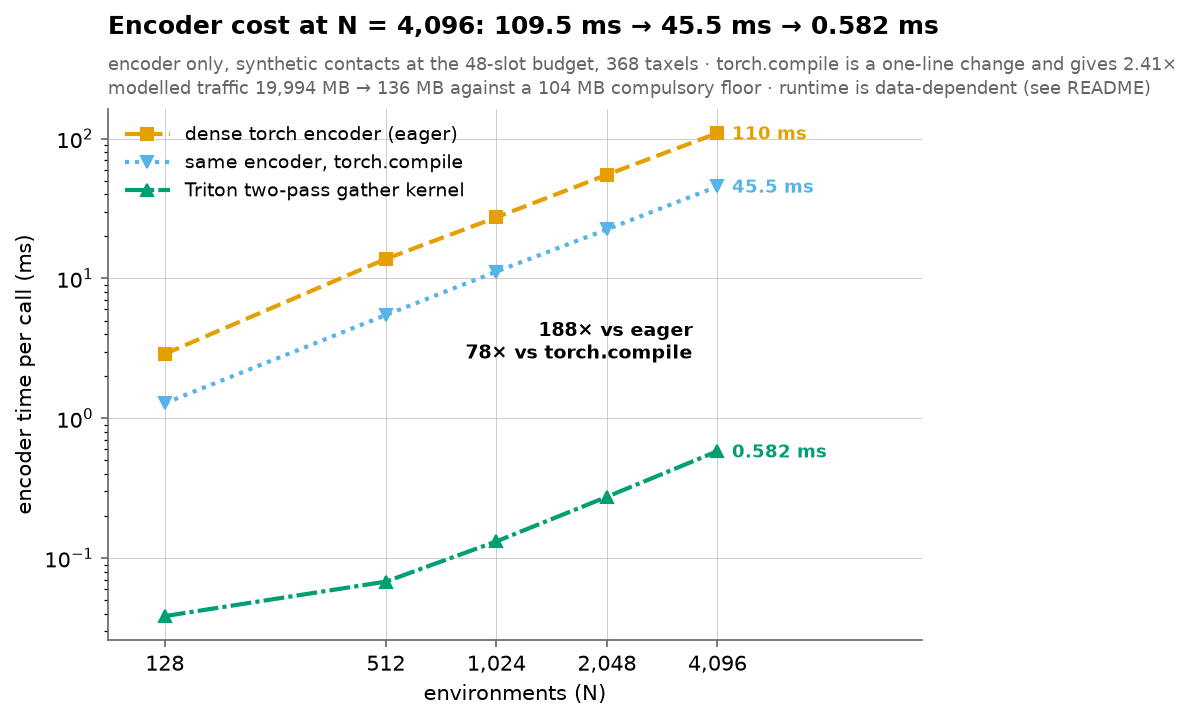
\includegraphics[width=\columnwidth]{F_encoder_three_ways.png}
  \caption{Isolated encoder latency for eager PyTorch, \texttt{torch.compile}, and Triton. Compilation is a strong one-line baseline, but sparsity and traffic avoidance dominate at scale.}
  \label{fig:threeways}
\end{figure}

\subsection{Kernel performance and correctness}

Table~\ref{tab:kernel} compares the three isolated implementations. At $N=4096$, Triton reduces runtime from 109.525~ms eager and 45.536~ms compiled to 0.582~ms: gains of 188 and 78 times, respectively. Modeled traffic falls to 136~MB against a 103.8~MB compulsory floor. Its modeled bandwidth is 233.8~GB/s, or 89.6\% of the empirical read ceiling. Peak PyTorch allocation falls from 4.095~GB to 0.183~GB.

\begin{table}[t]
\caption{Isolated encoder benchmark. Times are milliseconds per call; speedups use unrounded measurements.}
\label{tab:kernel}
\centering
\small
\begin{tabular}{rrrrrr}
\toprule
$N$ & Eager & Compile & Triton & vs. eager & vs. compile \\
\midrule
128  & 2.887  & 1.282  & 0.038 & 74.9$\times$ & 33.3$\times$ \\
1024 & 27.340 & 11.196 & 0.132 & 207.5$\times$ & 85.0$\times$ \\
4096 & 109.525& 45.536 & 0.582 & 188.2$\times$ & 78.3$\times$ \\
\bottomrule
\end{tabular}
\end{table}

Across 20 repeated runs at $B=1024$, all 1,130,496 output floats are bit-identical. This is run-to-run determinism, not bit equality with the CPU oracle. The maximum absolute error against the oracle fixture is $1.94\times10^{-6}$, and the kernel was re-gated inside the benchmark harness at $1.49\times10^{-7}$ before the end-to-end sweep.

\subsection{End-to-end effect and Amdahl's law}

At $N=4096$, the dense encoder's measured share $p=0.769$ gives an ideal end-to-end ceiling
\begin{equation}
  S_{\max}=\frac{1}{1-p}=4.34.
\end{equation}
The Triton path improves end-to-end throughput from 28,006 to 116,961 physics steps/s, a gain of 4.18, or 96\% of that available ceiling. Relative to 128,061 physics steps/s without tactile encoding, the cost of touch changes from $128061/28006=4.57$ to $128061/116961=1.09$. The encoder share falls to 6.5\%. Figures~\ref{fig:slowdown} and~\ref{fig:touchfree} show the result from complementary viewpoints; Fig.~\ref{fig:amdahl} places it against the bound.

\begin{table}[t]
\caption{End-to-end result at $N=4096$ and $\mathit{sim\_dt}=0.01$~s. Rates are physics steps/s.}
\label{tab:endtoend}
\centering
\small
\begin{tabular}{lrrr}
\toprule
Path & steps/s & Cost of touch & Encoder share \\
\midrule
Physics only & 128,061 & 1.00$\times$ & 0.0\% \\
Eager splat & 28,006 & 4.57$\times$ & 76.9\% \\
Triton splat & 116,961 & 1.09$\times$ & 6.5\% \\
\bottomrule
\end{tabular}
\end{table}

\begin{figure}[t]
  \centering
  
\includegraphics[width=\columnwidth]{D_slowdown_factor.png}
  \caption{Slowdown relative to physics-only execution. The eager tactile cost grows with batch size, whereas the Triton path remains close to the physics baseline.}
  \label{fig:slowdown}
\end{figure}

\begin{figure}[t]
  \centering
  
\includegraphics[width=\columnwidth]{E_touch_is_free.png}
  \caption{At $N=4096$, replacing the dense encoder changes the tactile overhead from a 4.57-fold step cost to 1.09-fold; ``nearly free'' here refers only to the measured simulator step.}
  \label{fig:touchfree}
\end{figure}

\begin{figure}[t]
  \centering
  
\includegraphics[width=\columnwidth]{H_amdahl.png}
  \caption{Measured end-to-end gain approaches the 4.34-fold ceiling set by the eager encoder's pre-optimisation share; further kernel tuning has little end-to-end leverage.}
  \label{fig:amdahl}
\end{figure}

\subsection{The kernel result under realistic grasp motion}
\label{sec:grasp}

The numbers above were taken at the frozen pose of Section~\ref{sec:motion}, where every world holds the same commanded grasp for the whole measurement. Because the Triton kernel's work is data-dependent while the dense baseline's is not, that operating point is a weak test by construction: it is a single, uniform, moderate contact regime. Repeating all three sweeps under the seven decorrelated grasp patterns tests whether the result survives a population in which some worlds are idle, some are at 25 contacts, and no two are alike.

It does. Table~\ref{tab:grasp} gives the comparison at $N=4096$. The dense baseline is unchanged at 4.58 against 4.57, and the Triton path measures 1.01 against 1.09; the encoder stage is 2.394~ms under motion against 2.432~ms frozen. The physics-only baseline itself falls 1.1\%, consistent with a slightly lower mean contact count (7.3 against 7.5).

\begin{table}[t]
\caption{Frozen pose versus scripted grasp motion at $N=4096$. Rates are physics steps/s; cost is relative to the physics-only run of the same motion condition.}
\label{tab:grasp}
\centering
\small
\begin{tabular}{lrrrr}
\toprule
 & \multicolumn{2}{c}{Frozen pose} & \multicolumn{2}{c}{Grasp motion} \\
\cmidrule(lr){2-3}\cmidrule(lr){4-5}
Path & Steps/s & Cost & Steps/s & Cost \\
\midrule
Physics only & 128,061 & 1.00$\times$ & 126,637 & 1.00$\times$ \\
Eager splat  & 28,006  & 4.57$\times$ & 27,642  & 4.58$\times$ \\
Triton splat & 116,961 & 1.09$\times$ & 125,535 & 1.01$\times$ \\
\bottomrule
\end{tabular}
\end{table}

That the Triton figure improves rather than degrades is a consequence of the kernel's decomposition, not a favourable draw. Pass 2 is indexed by environment--taxel tile: a program traverses its own environment's contact slots, finds them invalid, and exits the inner loop. An idle world therefore costs a scan of its slot array rather than a full evaluation, and because neither pass uses atomics or cross-world synchronisation, it does not hold up a loaded world either. Under motion many worlds are below the frozen pose's uniform occupancy, so the total work falls. The corollary from Section~\ref{sec:threats} still stands: a grasp that keeps every world near the 48-slot cap would cost more, and 1.01 should not be read as an upper bound on the kernel's cost.

The 1.01 figure is at the edge of what the harness resolves. At $N=1024$ the Triton path measures 76,891 against a physics-only 72,804, that is, nominally faster than doing no tactile work at all. The honest statement is that under grasp motion at large $N$ the Triton encoder's end-to-end cost is not distinguishable from run-to-run variation, not that it is exactly 1.01.

\subsection{The touch grid: the contacts are free, the budget is not}
\label{sec:grid}

The registered hypothesis for the geom-based touch grid predicted that it would degrade throughput from inside the physics step by inflating contact generation against a static budget, and that contacts would be silently dropped before throughput degraded noticeably. The conclusion is confirmed --- it costs 4.35 at $N=4096$, from inside physics --- but the mechanism is refuted, and the failure mode is worse than predicted. Both are worth stating plainly.

Two corrections come first. The grid is \textbf{300} patch geoms, not the 361 that a count of \texttt{\textless geom} lines in its XML suggests; that larger figure includes visuals, coarse collision boxes and class defaults. Measured on the compiled model the sensor grid is 300 geoms, taking the scene from 71 to 371. And ``silent dropping'' understates the failure: at the reference \texttt{nconmax}=48 / \texttt{njmax}=120, mujoco\_warp does not drop contacts and continue. It runs past its buffers and dies with \texttt{Warp CUDA error 700: illegal memory access} inside \texttt{ccd\_kernel}. The touch grid cannot be run at the reference budget at all. Measured against the CPU reference on a closing grasp, it requires \texttt{ncon}=232 and \texttt{nefc}=944 where the bare scene needs 24 and 112.

The contact explosion is intrinsic to the representation rather than an artifact of injecting patches into a model lineage they were not authored for. Classifying contacts by what they touch settles it: at the 232-contact peak, 223 are patch-versus-cube and none are patch-versus-patch, patch-versus-hand or patch-versus-floor. The swept runs agree at scale --- at $N=4096$, 139{,}102 of 161{,}832 live contacts involve a patch, and every one of those is against the cube. Three hundred small boxes tiling a hand against a cube simply generate an order of magnitude more simultaneous contacts than the hand's 37 coarse collision boxes do. Restricting the patches to collide only with the cube changes nothing, because they were never touching anything else.

The decomposition in Table~\ref{tab:grid} then locates the cost, and it is not where the hypothesis put it.

\begin{table}[t]
\caption{Touch-grid decomposition at $N=4096$. All rows use the same scene and timestep; only the geometry and the declared budget differ.}
\label{tab:grid}
\centering
\small
\begin{tabular}{lrrrr}
\toprule
Variant & Geoms & \texttt{ncon}/\texttt{njmax} & Steps/s & vs.\ bare \\
\midrule
Physics only        & 71  & 48 / 120   & 128,061 & --- \\
Grid, collisions off& 371 & 48 / 120   & 124,963 & $-$2.4\% \\
Grid, collisions off& 371 & 256 / 2048 & 28,926  & $-$77.4\% \\
Grid, cube only     & 371 & 256 / 2048 & 29,440  & $-$77.0\% \\
\bottomrule
\end{tabular}
\end{table}

Reading down the table: 300 extra collision geoms cost 2.4\%. Turning their collisions on with the budget held fixed costs nothing --- the cube-only row is if anything marginally faster than the non-colliding one, well inside run-to-run variation. The entire collapse sits between the second and third rows, which differ only in how much contact space was allocated. The same pair at $N=1024$ gives 81,741 against 24,889, a factor of 3.3, again with the live contact count pinned at roughly 7.4 per environment in both.

A dedicated budget scan separates the two allocations. Holding $N=1024$ and collisions off, so that occupancy is fixed, raising \texttt{njmax} from 120 to 2048 at \texttt{nconmax}=48 costs nothing (82,422 to 100,258 steps/s, the higher figure within noise), whereas raising \texttt{nconmax} from 48 to 256 at \texttt{njmax}=120 costs 82,422 down to 24,012, a factor of 3.4 with identical physics. \texttt{njmax} is not the parameter that costs; \texttt{nconmax} is.

Scanning \texttt{nconmax} alone establishes the shape of that cost. Figure~\ref{fig:budget} plots \texttt{benchmarks/contact\_budget\_sweep.py} over 48, 96, 128, 192, 256 and 384 slots per environment at $N=1024$, with \texttt{njmax}, the scene, the pose and the timestep all held fixed, so that the live contact count stays pinned between 7.4 and 7.7 per environment at every point and the allocation is the only thing that moves. Two series are run: the bare 71-geom scene, and the 371-geom touch grid with its collisions switched off. Least squares gives
\begin{equation}
  t_{\mathrm{step}} \approx 5.5 + 0.143\,\texttt{nconmax}\ \ \mathrm{ms}, \quad N=1024,
\end{equation}
on the bare scene ($R^{2}=0.998$), against $4.7 + 0.144\,\texttt{nconmax}$ on the grid series ($R^{2}=0.996$). The two slopes agree to 0.6\% across a fivefold difference in geometry count, which is the evidence that the cost attaches to the allocation and to nothing else. Throughput falls 78,045 to 17,062 steps/s across the scan, a factor of 4.6, with the same physics throughout. An earlier set of single-point runs at these conditions gave a slope of 0.145; the banked scan reproduces it to within 1\%.

\begin{figure}[t]
  \centering
  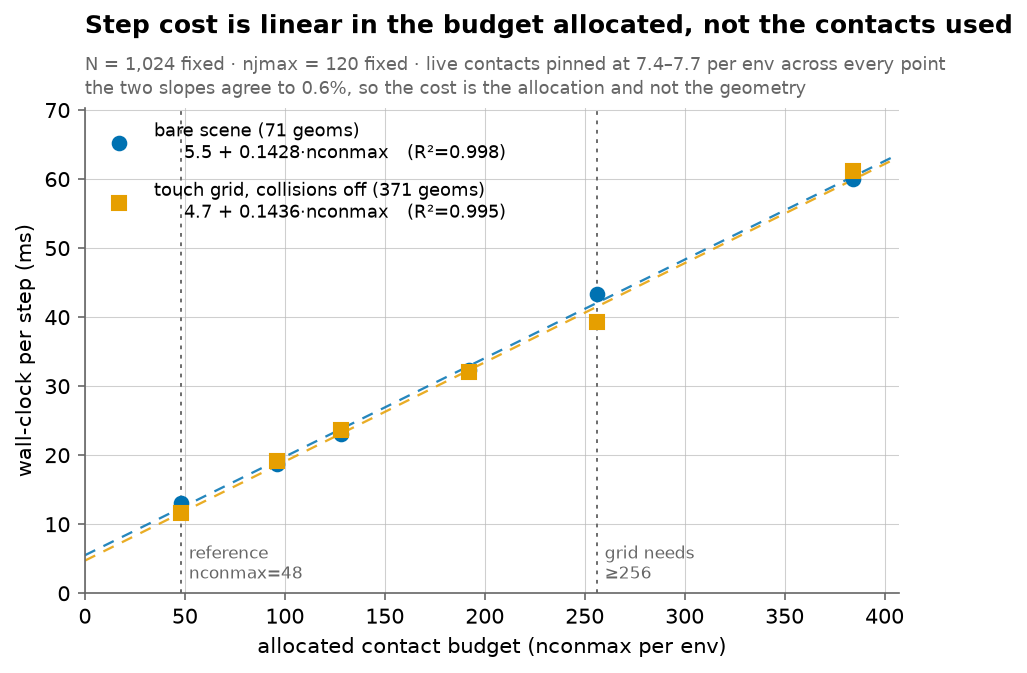
\includegraphics[width=\columnwidth]{J_contact_budget.png}
  \caption{Step time against the \emph{allocated} contact budget at $N=1024$, with the live contact count pinned at 7.4--7.7 per environment throughout. The bare scene and the 371-geom touch grid with collisions disabled give slopes agreeing to 0.6\%, so the cost follows the allocation rather than the geometry or the occupancy.}
  \label{fig:budget}
\end{figure}

The mechanism is visible in mujoco\_warp's source. Kernels are dispatched over \texttt{d.naconmax}, the allocation, rather than over the live contact count --- in collision detection, in constraint assembly, in sensor evaluation, and most expensively in \texttt{smooth.py}, whose launch is dimensioned \texttt{(m.nacttrnbody, d.naconmax, m.nv)}. Every step pays for every slot, whether or not a contact occupies it.

Two consequences follow, and the second is not specific to tactile sensing. Any tactile representation that forces the contact budget upward pays proportionally before it computes a single sensor value, which is the real and structural cost of the geom-based route. And \texttt{nconmax} is a first-class throughput parameter rather than a safety margin: at $N=1024$ the difference between 48 and 256 slots is 3.4-fold end to end with the same physics. Whether the reference \texttt{nconmax}=48 is deliberate and tight, or padded, is therefore worth confirming --- if padded, trimming it is free throughput, and if too tight for some grasp, the failure mode on GPU is a crash rather than a warning.

Under grasp motion the picture is the same but the budget question sharpens. The cube-only grid at $N=4096$ measures 27,942 steps/s against a moving physics-only baseline of 126,637, a cost of 4.53. Its peak per-world contact count rises to 390, against the 232 measured at the frozen closing grasp, with no overflow reported at the 256-slot-per-world allocation. The budget a geom-based grid requires is therefore a property of the motion, not of the pose one happens to benchmark, and sizing it from a static grasp will under-provision it.

The registered prediction that this would be ``a correctness problem presenting as a performance one'' was right in spirit and wrong in mechanism. It is both a correctness problem and a performance problem, but they are not the same effect: the crash comes from real contacts overrunning the budget, and the slowdown comes from the allocation made to prevent the crash.

\subsection{Flex: viable on Warp, two orders of magnitude too slow}
\label{sec:flex}

The flex representation was registered as a stretch hypothesis --- viable on Warp but impractical at scale --- with the expectation that it would fail by exhausting the Spark's unified memory. Both halves of the conclusion hold and the predicted failure mode does not.

Viability is confirmed concretely: \texttt{mjw.put\_model} accepts the flex model without complaint. That is the direct evidence for the project's premise that flex tactile is GPU-viable under Warp, where the JAX backend raises \texttt{NotImplementedError} for flex outright. \texttt{put\_data} then requires \texttt{njmax} $\geq 3030$ per world and says so cleanly, as a \texttt{ValueError} at allocation time. The contrast with the touch grid is worth keeping: the same class of budget shortfall announces itself politely in one path and fatally inside a CUDA kernel in the other, which suggests the touch-grid crash is a robustness gap in mujoco\_warp rather than an inherent property of overrunning a budget.

Cost must be quoted at matched simulated time, not per step. The flex model declares \texttt{timestep}=0.002~s with 50 solver iterations and does not survive the rigid sweeps' 0.01~s: forced to it, MuJoCo reports \texttt{Nan, Inf or huge value in QACC} and the Kelvin--Voigt readout returns forces of order $10^5$~N. An earlier version of this measurement made exactly that error, and its figures are superseded here. Since a 0.002~s step advances one fifth as far, raw step rates overstate flex fivefold against the rigid sweeps. Gripping, at \texttt{njmax}=4096: $N=1$ costs 137.1~ms per step (1 equivalent env-step/s against the rigid hand's 308), $N=64$ 256.9~ms (50 against 15{,}999, a factor of 320), and $N=256$ 719.2~ms (71 against 38{,}310, a factor of 540). Solver iterations are not the driver --- 50 versus 5 iterations differ by 0.4\% --- the timestep is.

More decisive than the ratio is that flex saturates early: equivalent throughput moves only from 50 to 71 env-steps/s between $N=64$ and $N=256$ while per-step latency nearly triples, and a separate run at the larger timestep was flat from $N\approx128$ with latency thereafter scaling exactly linearly --- a fully saturated device rather than a launch-bound one. The rigid hand is still gaining throughput from $N=1024$ to $N=4096$. Reaching training scale is therefore not a matter of waiting longer or finding a larger machine.

Ablation at $N=64$ locates the cost: disabling the constraint solver removes 37\%, disabling contacts removes 1\%, and the remaining 63\% is forward dynamics over 387 bodies and 1120 degrees of freedom. Touch is almost irrelevant to it. No kernel of ours can help, because all of it lies inside \texttt{mjw.step}; the Kelvin--Voigt readout this project would control is a few thousand floating-point operations against roughly 200~ms.

Memory never bound: peak resident set is 0.75~GB at $N=1$ and 1.22~GB at $N=1024$. This is the second measurement in this project to find the unified-memory ceiling irrelevant to the simulation itself, the first being bare physics at 4096 environments in 0.92~GB. The model is simply expensive to integrate --- 1120 degrees of freedom and 386 equality constraints per hand, solved every step. The flex skin's own taxel readout was not measured, on the grounds that the physics alone is already two orders of magnitude over budget and no readout cost could change the conclusion.

\subsection{The encoder inside the reference training environment}
\label{sec:mjlab}

Every figure above prices a bare \texttt{mjw.step} loop. That isolates the representations from one another, which is what a comparison needs, but it omits everything a training run also pays for: observation, reward, termination and command managers, episode resets, domain randomisation, and five physics steps per control step. To close that gap the splat encoder was wired into \texttt{leapXelaMjLab} itself, as an \texttt{ObservationTermCfg} beside the existing joint and cube terms, and the environment timed through its own \texttt{ManagerBasedRlEnv}.

Three integration hazards are worth recording, because each fails silently or fatally rather than visibly. First, mjlab namespaces scene elements by entity: bodies become \texttt{robot/palm}, the manipulated cube's geom \texttt{cube/cube}, injected sites \texttt{robot/taxel\_017}. A layout carrying bare names matches nothing, which is the all-zero failure mode this project has guarded against throughout; it surfaces as an exception only because \texttt{prepare\_static} raises on a failed lookup. Second, the taxel layout's entries are frozen dataclasses, so the prefix rewrite must rebuild rather than mutate. Third, and least obvious: the benchmark harness puts Warp on torch's stream to order the encoder behind the physics, which is correct when the harness owns the Warp context, and is a segmentation fault inside mjlab. \texttt{Simulation.\_\_init\_\_} captures step, forward, reset and sense into CUDA graphs bound to the Warp stream current at capture time, and observation terms are constructed afterwards; repointing the stream underneath a captured graph crashes the process. Ordering torch behind Warp with an event instead costs 0.02~ms and is safe.

The measured cost is reported twice, because the environment as shipped contains an unrelated inefficiency large enough to dominate it (\S\ref{sec:upstream}). At $N=2048$, without tactile the environment steps in 16.16~ms; with 368 taxels it steps in 50.70~ms, a factor of 3.14. Direct measurement shows the encoder is not responsible: \texttt{encode()} alone takes 1.26~ms, matching the harness at the same $N$, the observation term is invoked once per environment step, and the stream ordering costs 0.02~ms. With the upstream inefficiency patched the same environment costs 14.05~ms without tactile and 16.67~ms with it --- a factor of \textbf{1.19}, against the 1.17 the harness predicted at the same env count. The isolated benchmark therefore transfers.

Two caveats bound that number in opposite directions, and neither is small. No policy or optimiser is running: actions are a fixed tensor, so the tactile share reported here is an upper bound on its share of real training, which has a larger denominator. Against that, an untrained policy drops the cube frequently, while a trained one grips deliberately and sustains far more contact --- and the Triton kernel's cost tracks live contact count, from 0.54~ms at one contact per environment to 1.27~ms with the budget saturated. The cost of tactile sensing during training is therefore not a constant but a function of how well the policy has learned to hold the object, rising as it improves.

\section{Threats to Validity}
\label{sec:threats}

\textit{Profiler access.} Nsight Compute was blocked by \texttt{ERR\_NVGPUCTRPERM}: the driver restricts profiling counters to administrators. There is therefore no Nsight-reported limiter and no Nsight-measured DRAM throughput anywhere in this work. The roofline uses the empirically measured 260.8~GB/s read and 18.44~TFLOP/s SGEMM ceilings, while achieved bandwidth is computed from modeled bytes and measured time. In particular, apparent 96--99\% bandwidth utilisation at intermediate $N$ probably charges L2 reuse as though it were DRAM traffic. The 89.6\% result at $N=4096$ is the defensible figure.

\textit{Contact dependence.} The dense baseline has fixed work for its padded shape, but the sparse kernel is data-dependent. At $N=4096$ it takes 0.54, 0.57, and 1.27~ms at 1, 4.3, and 48 live contacts per environment, respectively. Section~\ref{sec:grasp} retires the narrower version of this concern --- that the headline came from a single frozen pose in which every world was identical --- since the result survives a decorrelated population spanning 0 to 25 contacts per world. What remains is the upper end: no measured condition holds every world near the 48-slot cap, and the fully occupied synthetic case, while still 86 times faster than eager, is 2.2 times slower than the measured regime. A grasp that saturates the budget would cost more than 1.01.

\textit{Cross-representation comparability.} Native touch, the splat and the touch grid are measured in the same pinned scene at the same timestep, so Table~\ref{tab:fourways} compares them directly. Flex is not: it is a different body tree in a different model lineage, and no injection converts one into the other. Its per-step latency is a fair same-engine order-of-magnitude comparison and its throughput is not a like-for-like fourth measurement, which is why it appears in that table with a ratio rather than a rate. Separately, the touch grid is quoted at \texttt{nconmax}=256 because it cannot run at 48; part of its cost is therefore a budget the other rows do not pay, which is the finding of Section~\ref{sec:grid} rather than a confound, but the rows are not held at a common allocation.

\textit{Motion coverage of the other representations.} The grasp-motion re-run covers physics-only, both splat paths, the touch grid and native touch; flex is the one representation priced only at a held grip, and its margin is such that no motion could close it. The native-touch sweep required a harness fix before it would run: its verification gate sampled a single instant and aborted at $N=1$ because all 421 sensors read zero at that instant. That was a false alarm rather than a broken readout --- the \texttt{tap} pattern deliberately releases toward the pregrip pose at 1.5~Hz, and at $N=1$ there is one world running one pattern at one phase, so a quiet frame means an open hand. The gate now samples a window and takes the best frame, which still catches a sensor array that never fires. What remains a genuine limit is resolution rather than coverage: as recorded above, native touch's cost under motion is bounded at 1.08 but not resolved, because the effect stays comparable to run-to-run variation.

\textit{Oracle coverage and geometry.} The oracle fixture was widened from a single scripted grasp to 632 frames over 56 trials of the seven grasp patterns, raising the taxels that ever fire from 37 to 176 of 368 and the fingertip coverage from 2 to 57 of 136. Both implementations still validate. Widening it exposed two properties of the reference algorithm rather than of this port. First, the encoder's splat gates are hard thresholds followed by renormalisation over the surviving weights, and in this scene the palm taxel plane sits at $|z|=10.0000$~mm against a 10~mm cutoff, with margins of 0 to 0.2~$\mu$m. Single precision cannot resolve that, so a taxel can fall on the opposite side of the gate from the double-precision reference and rescale the survivors, producing a clean 4.6\% relative difference on loaded palm taxels; the same code in double precision collapses the error to $4.16\times10^{-7}$. Any single-precision GPU port of this encoder will show that disagreement, and it is a property of the gate, not of the kernel. Second, 48 medial taxels are structurally unreachable in this scene: every cube contact on the medial links is 11.50~mm out of plane, a constant above the 10~mm cutoff, and no motion fixes it because the pads sit on a different face of the link from the one the cube presses. This was verified to be a property of the layout rather than of the transplant, since taxel-to-surface geometry is identical in both lineages. Separately, 136 taxels lie on four fingertips whose RL-lineage geometry is approximately 10.3~mm longer than the tactile lineage; their contacts straddle the gate at 9 to 10.8~mm and a third to a half of them produce nothing. Comparing the mesh assets directly localises this to a single revised part rather than a general modelling divergence, as described in Section~\ref{sec:method-model}, which is why it is stated here as a question with an answer rather than as an inherent limit. Correctness against the software oracle establishes implementation fidelity, not complete physical validity.

\textit{System boundary.} The benchmark measures physics plus the tactile stage, not the full mjlab training loop. It excludes PPO, policy evaluation, other observations, reward computation, rollout storage, and resets. All four representations are now priced against each other at the simulator step, but none has been priced with a policy attached.

\textit{Configuration caveat.} At the 0.01~s timestep, between 1 and 3 of 4096 worlds raise \texttt{OverflowType.NEFC} depending on the run, at most 0.073\%. Warp requests \texttt{njmax}=124 against the configured 120. Contacts are unaffected: the observation is 7.1 contacts per environment against a cap of 48. This is constraint-row overflow rather than contact overflow, and the harness's aggregate overflow field must not be interpreted as a dropped-contact count.

\begin{figure}[t]
  \centering
  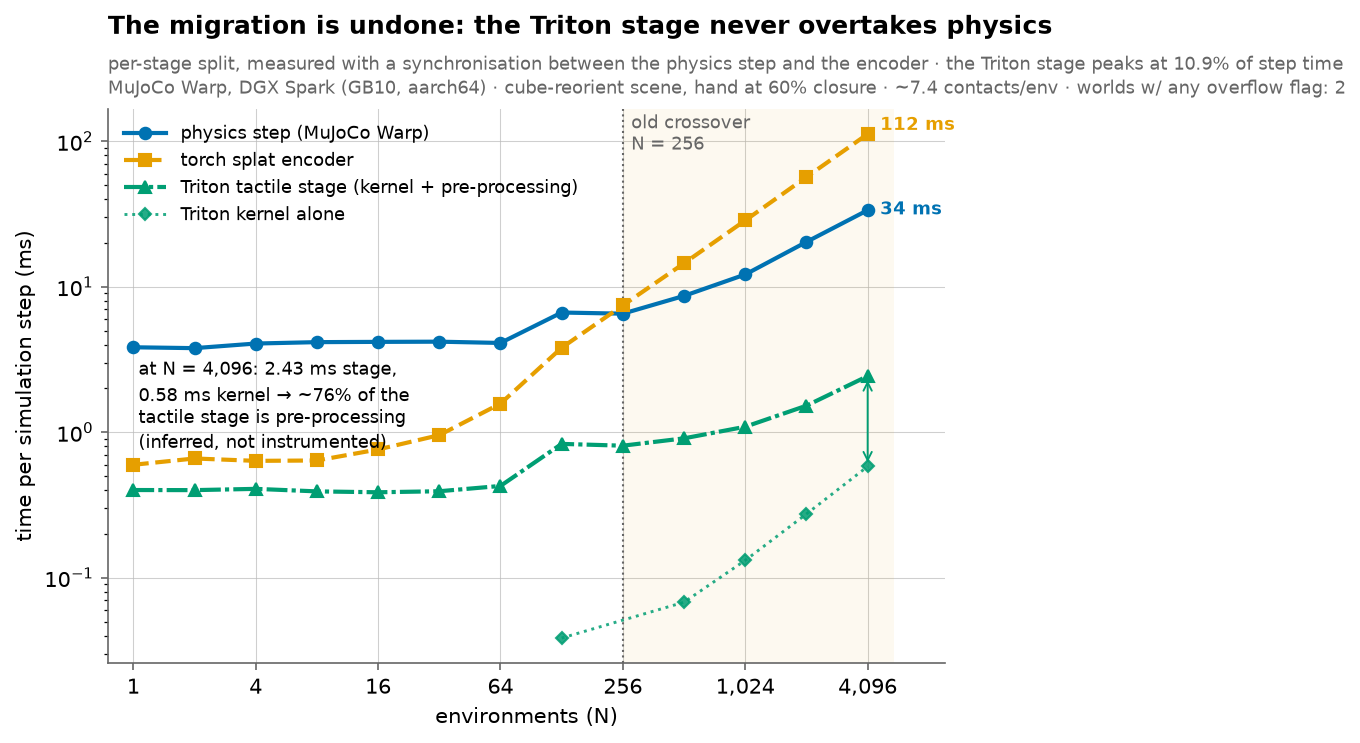
\includegraphics[width=\columnwidth]{G_migration_undone.png}
  \caption{The optimised encoder reverses the first bottleneck migration, but the remaining tactile-stage overhead motivates measurement inside preprocessing.}
  \label{fig:undone}
\end{figure}

\section{Incidental Findings for Upstream}
\label{sec:upstream}

Four observations should be reported independently of the encoder result.

\textit{\texttt{nconmax} is a throughput parameter.} This is the most valuable of the three and is not specific to tactile work. Because mujoco\_warp dispatches over the allocated contact budget rather than the live count, step time is affine in \texttt{nconmax} at fixed occupancy, and the difference between 48 and 256 slots is 3.4-fold end to end at $N=1024$. Any Warp configuration therefore wants its contact budget audited as a performance setting: padding it is not free, and the cost is invisible in the contact statistics. Whether the reference \texttt{nconmax}=48 is deliberate or a placeholder is worth settling for that reason alone.

\textit{Budget overrun is not reported gracefully in contact detection.} Overrunning \texttt{njmax} at allocation time produces a clean \texttt{ValueError} naming the required value. Overrunning the contact budget at run time produced an illegal memory access inside \texttt{ccd\_kernel} instead. The asymmetry looks like a robustness gap rather than an inherent property, and it is the difference between a configuration error a user can read and a crash they must bisect.

\textit{An mjlab accessor computes and discards orientations.} \texttt{EntityData.site\_pos\_w} returns \texttt{site\_pose\_w[..., 0:3]}, and \texttt{site\_pose\_w} gathers every site's position and $3\times3$ orientation, applies \texttt{quat\_from\_matrix} to all of them, concatenates an $(N, \mathrm{nsite}, 7)$ tensor, and then three columns are sliced out and the quaternions discarded. The reference task performs this twice per step to obtain one site's position and four sites' positions respectively. With the stock hand's 68 sites the waste is small; with 368 taxel sites injected it becomes the largest single cost in the environment. Reading positions directly reduces the step from 49.92 to 15.07~ms at $N=2048$, a factor of 3.31, and also improves the no-tactile environment from 16.16 to 14.05~ms --- which establishes that the cost is not caused by tactile sensing but merely exposed by it. The substitution is exact rather than approximate: slicing the first three columns from a concatenation whose first three columns are the positions is the identity, verified bitwise over $64\times435\times3$ values, with step-zero observations identical and no in-place writes to the property anywhere in the codebase. The same pattern appears in six property pairs, of which the site and geom variants are the expensive ones.

\textit{The marginal \texttt{njmax} setting.} At the supervisor's timestep, the configured 120 constraint rows are insufficient in 1 to 3 of 4096 worlds depending on the run, and Warp asks for 124. Contact occupancy remains far below its separate cap, so the relevant action is auditing the constraint-row budget. The low incidence makes this minor in the present benchmark, but silent overflow in a training configuration warrants review. The harness's aggregate overflow field counts any overflow bit and must not be read as a dropped-contact count.

\section{Future Work}

With all four representations priced, the open work is no longer breadth but depth.

The next optimisation target is tactile preprocessing, not the Triton kernel. In the current $N=4096$ sweep the complete tactile stage is 2.432~ms, whereas the isolated kernel is 0.582~ms. Subtracting these separately timed measurements suggests that approximately 76\% of the stage lies in contact-force extraction and packing. This is an inference, not direct instrumentation, so the stage must be subdivided and measured before attributing the residual to individual operations. Figure~\ref{fig:undone} illustrates this second prospective bottleneck migration.

The optimised observation should then be wired into the full mjlab loop and evaluated with the policy, PPO, rewards, resets, and rollout buffers active. Only that measurement converts the cost-of-sensing table into a cost-of-training statement, and the conversion is not a simple division: the control decimation of five means the tactile stage is amortised over five physics steps if the observation is read once per control step rather than once per physics step, which no measurement here assumes.

One smaller item follows from the new results. The contact-budget law now has a banked sweep and two agreeing series behind it, but both were taken at a single environment count on a single scene. Its slope is the quantity a user would actually want, and whether that slope is a constant of the machine, a function of $N$, or a function of the model's degrees of freedom is not established here. The same scan across several environment counts and at least one unrelated scene would settle it, and is cheap.

Finally, the physical fingertip variant must be established and the 136 lateral placements either validated or re-projected. The widened oracle now exercises 57 of those taxels, which is enough to show the geometry is marginal and not enough to fix it.

\section{Conclusion}

Four ways of sensing touch in a GPU-parallel simulator were priced at training scale, and they differ by more than two orders of magnitude for reasons that are structural rather than incidental. Native \texttt{\textless touch\textgreater} is essentially free and already on GPU. The deformable flex skin is roughly 540 times the cost of the rigid hand at matched simulated time and has saturated by 256 environments, so it is out of reach by margins that no engineering closes. The geom-based touch grid and the faithful Gaussian splat both cost about four and a half times a bare step, but for unrelated reasons, and only one of them is fixable from a kernel.

The splat's cost was the fixable one, and its character changed as parallelism grew: a modest small-batch tax became the majority of step time once physics had amortised across hundreds of environments. Profiling showed the cause was neither GPU arithmetic nor launch overhead but dense traffic for mostly irrelevant contact--taxel pairs. A two-pass gather reformulation, constrained by the per-contact taxel normalisation, removed those intermediates while retaining deterministic semantics; it captured 96\% of the available Amdahl speedup and reduced the cost of touch from 4.57 to 1.09 times the physics-only step, and to 1.01 under scripted grasp motion.

The touch grid's cost was not fixable, and understanding why produced the result most likely to outlive this project. Its extra contacts are nearly free; what is expensive is the contact budget that must be allocated to hold them, because mujoco\_warp dispatches over the allocation and not the occupancy. That makes \texttt{nconmax} a throughput parameter worth 3.4-fold at 1024 environments, penalises any representation that inflates the contact set before it computes a single value, and applies to every Warp workload, tactile or not. The registered hypothesis that predicted this cost got the conclusion right and the mechanism wrong, which is recorded here rather than quietly amended.

The claims are limited to the simulator step. All four representations are now priced against each other there; none has been priced with a policy, an optimiser and rollout buffers attached, and that remains the measurement that would turn a cost of sensing into a cost of training.

\section*{Acknowledgements}

The author thanks Hamid (Mohammad Hamid, \url{https://github.com/mohammad200h}) for the LeapXELA hand model, the touch-sensor and touch-grid model variants, the mjlab reinforcement-learning training stack, and the seven grasp patterns of \texttt{sparsh-skin-sim}, whose constants are used verbatim in the motion driver of Section~\ref{sec:motion}.

The CPU reference encoder \texttt{VirtualTaxelSensor} (\texttt{leapxela/touch\_sensor.py}) is the work of Pratik Ingle (\texttt{pratik-ingle}), contributed in commit \texttt{5f305a8} on 3 August 2026; earlier drafts of this report attributed it to Hamid, which was incorrect. It is the semantic oracle for everything measured here, so the attribution matters.

The model reconciliation, GPU batched baseline, profiling study, Triton reformulation, representation harnesses, validation, and measurements reported here are the work of this project.

\appendices
\section{Reproducibility}

The measured software environment was MuJoCo 3.11.0, MuJoCo Warp 3.11.0, warp-lang 1.16.0, PyTorch 2.13.0+cu130, NumPy 2.5.2, CUDA 13.0.88, and Python 3.12.3 on an aarch64 GB10 with 48 streaming multiprocessors. Each command is executed from the repository root. The four shell variables below are shorthand for boilerplate every invocation repeats: the module search path, the memory-capped scope every run is launched under, and the interpreter.

{\footnotesize
\begin{verbatim}
PP=src:explore:third_party/leapXELA_model
CAP="systemd-run --user --scope -q"
MEM="-p MemoryMax=8G -p MemorySwapMax=0"
PY=.venv/bin/python
\end{verbatim}
}

Correctness gates first. These two were re-run while preparing this revision and pass 11 of 11; the 4096-environment sweeps below are the banked runs and were not repeated.

{\footnotesize
\begin{verbatim}
PYTHONPATH=$PP $CAP $MEM $PY \
  tests/test_encoder_oracle.py

PYTHONPATH=$PP $CAP $MEM $PY \
  tests/test_triton_kernel.py
\end{verbatim}
}

The profiling run behind Section~\ref{sec:profiling}:

{\footnotesize
\begin{verbatim}
PYTHONPATH=$PP $CAP $MEM $PY \
  profiling/profile_encoder.py \
  --mode bench --num-envs 4096 --bandwidth
\end{verbatim}
}

One point of each representation's sweep, at the largest environment count. The full ladders come from \texttt{scale\_sweep.py} below.

{\footnotesize
\begin{verbatim}
PYTHONPATH=$PP $CAP $MEM $PY \
  benchmarks/harness.py \
  --num-envs 4096 --tactile none

PYTHONPATH=$PP $CAP $MEM $PY \
  benchmarks/harness.py \
  --num-envs 4096 --tactile splat \
  --encoder torch

PYTHONPATH=$PP $CAP $MEM $PY \
  benchmarks/harness.py \
  --num-envs 4096 --tactile splat \
  --encoder triton --verify

PYTHONPATH=$PP $CAP $MEM $PY \
  benchmarks/harness.py \
  --num-envs 4096 --tactile touch \
  --touch-scene inject

PYTHONPATH=$PP $CAP $MEM $PY \
  benchmarks/harness.py \
  --num-envs 4096 --tactile touchgrid \
  --touchgrid-collide object \
  --nconmax-per-env 256 \
  --njmax-per-env 2048
\end{verbatim}
}

The contact-budget scan of Fig.~\ref{fig:budget}, both series. Each holds $N$ and \texttt{njmax} fixed and varies only the allocation:

{\footnotesize
\begin{verbatim}
$PY benchmarks/contact_budget_sweep.py \
  --tactile none --tag none_n1024

$PY benchmarks/contact_budget_sweep.py \
  --tactile touchgrid \
  --touchgrid-collide off \
  --tag grid_off_n1024
\end{verbatim}
}

The same splat point under the grasp motion of Section~\ref{sec:motion}, and the flex probe, which is a separate script because flex is a different body tree:

{\footnotesize
\begin{verbatim}
PYTHONPATH=$PP $CAP $MEM $PY \
  benchmarks/harness.py \
  --num-envs 4096 --tactile splat \
  --encoder triton --motion grasp \
  --verify

PYTHONPATH=$PP $CAP $MEM $PY \
  benchmarks/flex_probe.py \
  --num-envs 1024 --njmax 4096
\end{verbatim}
}

For a complete sweep, \texttt{benchmarks/scale\_sweep.py} launches one capped child per environment count and accepts the same \texttt{--tactile}, \texttt{--touchgrid-collide}, \texttt{--nconmax-per-env}, \texttt{--njmax-per-env} and \texttt{--motion} flags; the model timestep must be explicitly fixed at 0.01~s and outputs should be given the \texttt{\_dt01} suffix so they cannot be confused with the superseded 0.001~s data. The banked results underlying this report, all in \texttt{benchmarks/results/}, are:

{\footnotesize
\begin{verbatim}
kernel_bench.csv
scale_sweep_physics_only_dt01.csv
scale_sweep_splat_dt01.csv
scale_sweep_splat_triton_dt01.csv
scale_sweep_touch_dt01.csv
scale_sweep_touchgrid_off_dt01.csv
scale_sweep_touchgrid_off_bigbudget_dt01.csv
scale_sweep_touchgrid_object_dt01.csv
scale_sweep_grasp_physics_only_dt01.csv
scale_sweep_grasp_splat_dt01.csv
scale_sweep_grasp_splat_triton_dt01.csv
scale_sweep_grasp_touch_dt01.csv
scale_sweep_grasp_touchgrid_object_dt01.csv
contact_budget_none_n1024.csv
contact_budget_grid_off_n1024.csv
\end{verbatim}
}

The \texttt{nconmax} scan of Section~\ref{sec:grid} is banked as the two \texttt{contact\_budget} files above. The touch-grid budget isolation of that section and the flex latencies of Section~\ref{sec:flex} remain single-point runs rather than banked sweeps; their measurements are recorded in the project's hypothesis register under H3 and H4 respectively.

\end{document}
